\documentclass{beamer}
\usetheme{uic}
\usepackage{ctex}
\usepackage{amsfonts,amsmath,oldgerm,algorithmic,algorithm}
\usepackage[font=small,labelfont=bf]{caption} % Required for specifying captions to tables and figures

\newcommand{\hrefcol}[2]{\textcolor{uihteal}{\href{#1}{#2}}}
\newcommand{\testcolor}[1]{\colorbox{#1}{\textcolor{#1}{test}}~\texttt{#1}}

% Please see Section 18.1 of Beamer User Guide for all the options \usefonttheme provides
\usefonttheme[onlymath]{serif}
% \usefonttheme{serif} % use this if you would like Serif font throughout (and not just for math)

\title{基于SpringBoot \& Vue的在线考试系统}


\titlebackground*{images/uic_lockup.png}

% NOTE 1: The asterisk splits the background image. This option is good
% for logo-based backgrounds. If you use an image based background
% it's recommended to not split it:

% \titlebackground{images/uic_seo.jpg}

% NOTE 2: If you use a title background that does not have a logo, you might
% want to enable logo in the top left.
% To do that, simply comment out this line
\themecolor{lightnologo}

\subtitle{Using \LaTeX\ to prepare slides}
% This can be adjusted accordingly for longer titles
\newcommand{\titleboxwidth}{0.45\textwidth}

\author{\href{mailto:umunee2@uic.edu}{胡翌晨、张家瑞、王紫菱}}
\date{\today}

\begin{document}
\maketitle
\themecolor{light} % reverts to a logo based theme (if you disabled it for title page)a

% default is no footline, but page numbers are incredibly useful for the audience to ask questions later
\footlinecolor{uicblue}

\begin{chapter}[images/uic_halls.jpg]{uicblue}{项目概述}
\end{chapter}

\begin{frame}[fragile]{组员分工}
\begin{itemize}
    \item \textbf{胡翌晨}\\
    \qquad 服务器搭建、程序测试、视频制作、后端代码编写
    \item \textbf{张家瑞}\\
    \qquad 项目文档编写、程序测试、PPT制作
    \item \textbf{王紫菱}\\
    \qquad 前端设计、程序设计、PPT制作
\end{itemize}
\end{frame}


\begin{frame}[fragile]{项目概述}
\begin{itemize}
    \item 在线考试系统是一种基于互联网的教育技术工具,旨在为学生、教师或培训机构提供便捷的考试和评估方式。该系统基SpringBoot+Vue,结合了后端和前端的强大功能,提供了稳定、高效的用户体验
    \item 该系统的后端的 SpringBoot 框架具备快速开发和简化配置的特点,它实现了用户管理、考试管理、试卷管理和成绩管理等核心功能,同时集成了 Spring Security 来确保用户身份验证和权限管理的安全性
    \item 前端则采用了 Vue.js 框架,拥有响应式和组件化的特点,提供了流畅的用户界面和良好的交互体验。它实现了用户登录、考试列表、试卷详情、成绩查询等功能,利用 Vue Router 实现了页面路由,实现了单页面应用的效果,同时结合了Element UI 等 UI 组件库来美化页面样式,并提供丰富的交互组件
\end{itemize}
\end{frame}

\begin{chapter}[images/uic_halls.jpg]{uicblue}{系统分析}
\end{chapter}

\begin{frame}[fragile]{View 视图层}
作用:
    \begin{itemize}
    \item 用户界面的展示和交互
    \item 接收用户的输入操作
    \item 将用户操作传递给控制器处理
    \end{itemize}
特征:
    \begin{itemize}
    \item HTML、Vue.js等前端技术。
    \item 负责呈现数据和收集用户输入。
    \item 不包含业务逻辑,专注于界面和用户交互。
    \end{itemize}
\end{frame}

\begin{frame}[fragile]{Controller 控制器层}
作用:
    \begin{itemize}
    \item 处理用户的请求和操作。
    \item 调度和协调系统中的其他组件。
    \item 通常负责路由和请求转发。
    \end{itemize}
特征:
    \begin{itemize}
    \item Spring、Servlet等框架中的控制器。
    \item 接收来自视图层的请求并调用相应的服务层处理业务逻辑。
    \item 处理输入验证和参数校验,确保传递给服务层的数据有效性。
    \end{itemize}
\end{frame}
    
\begin{frame}[fragile]{Service 服务层}
作用:
    \begin{itemize}
    \item 执行业务逻辑和数据处理。
    \item 作为控制器和数据访问层(DAO层)之间的中介。
    \item 可以跨多个控制器共享。
    \end{itemize}
特征:
    \begin{itemize}
    \item Java类或者Spring的@Service注解类。
    \item 包含业务规则的实现,如数据处理、转换、验证等。
    \item 不直接与用户界面交互,而是接受控制器层传递的请求并返回处理结果。
    \end{itemize}
\end{frame}
        
\begin{frame}[fragile]{DataBase 数据访问层}
作用:
    \begin{itemize}
    \item 负责与数据库的交互。
    \item 执行数据的CRUD操作(创建、读取、更新、删除)。
    \item 提供持久化机制,确保数据的安全性和一致性。
    \end{itemize}
特征:
    \begin{itemize}
    \item DAO(Data Access Object)接口或者实现类。
    \item 使用JDBC、Hibernate、Spring Data等技术实现与数据库的通信。
    \item 负责处理数据库连接、事务管理、数据检索和更新等操作。
    \end{itemize}
\end{frame}

\begin{chapter}[images/uic_halls.jpg]{uicblue}{项目功能展示}
\end{chapter}

\begin{frame}[fragile]{需求概述}
\begin{itemize}
    \item \textbf{学生}\\
    \qquad 使用在线考试系统进行考试和学习的注册用户
    \item \textbf{教师}\\
    \qquad 负责管理和监督学生考试以及题库内容的用户
    \item \textbf{管理员}\\
    \qquad 系统的管理者,负责整体系统的配置、维护和用户管理
\end{itemize}
\end{frame}


\begin{frame}[fragile]{功能展示}
\framesubtitle{用户登录界面}
\begin{figure}
    \centering
    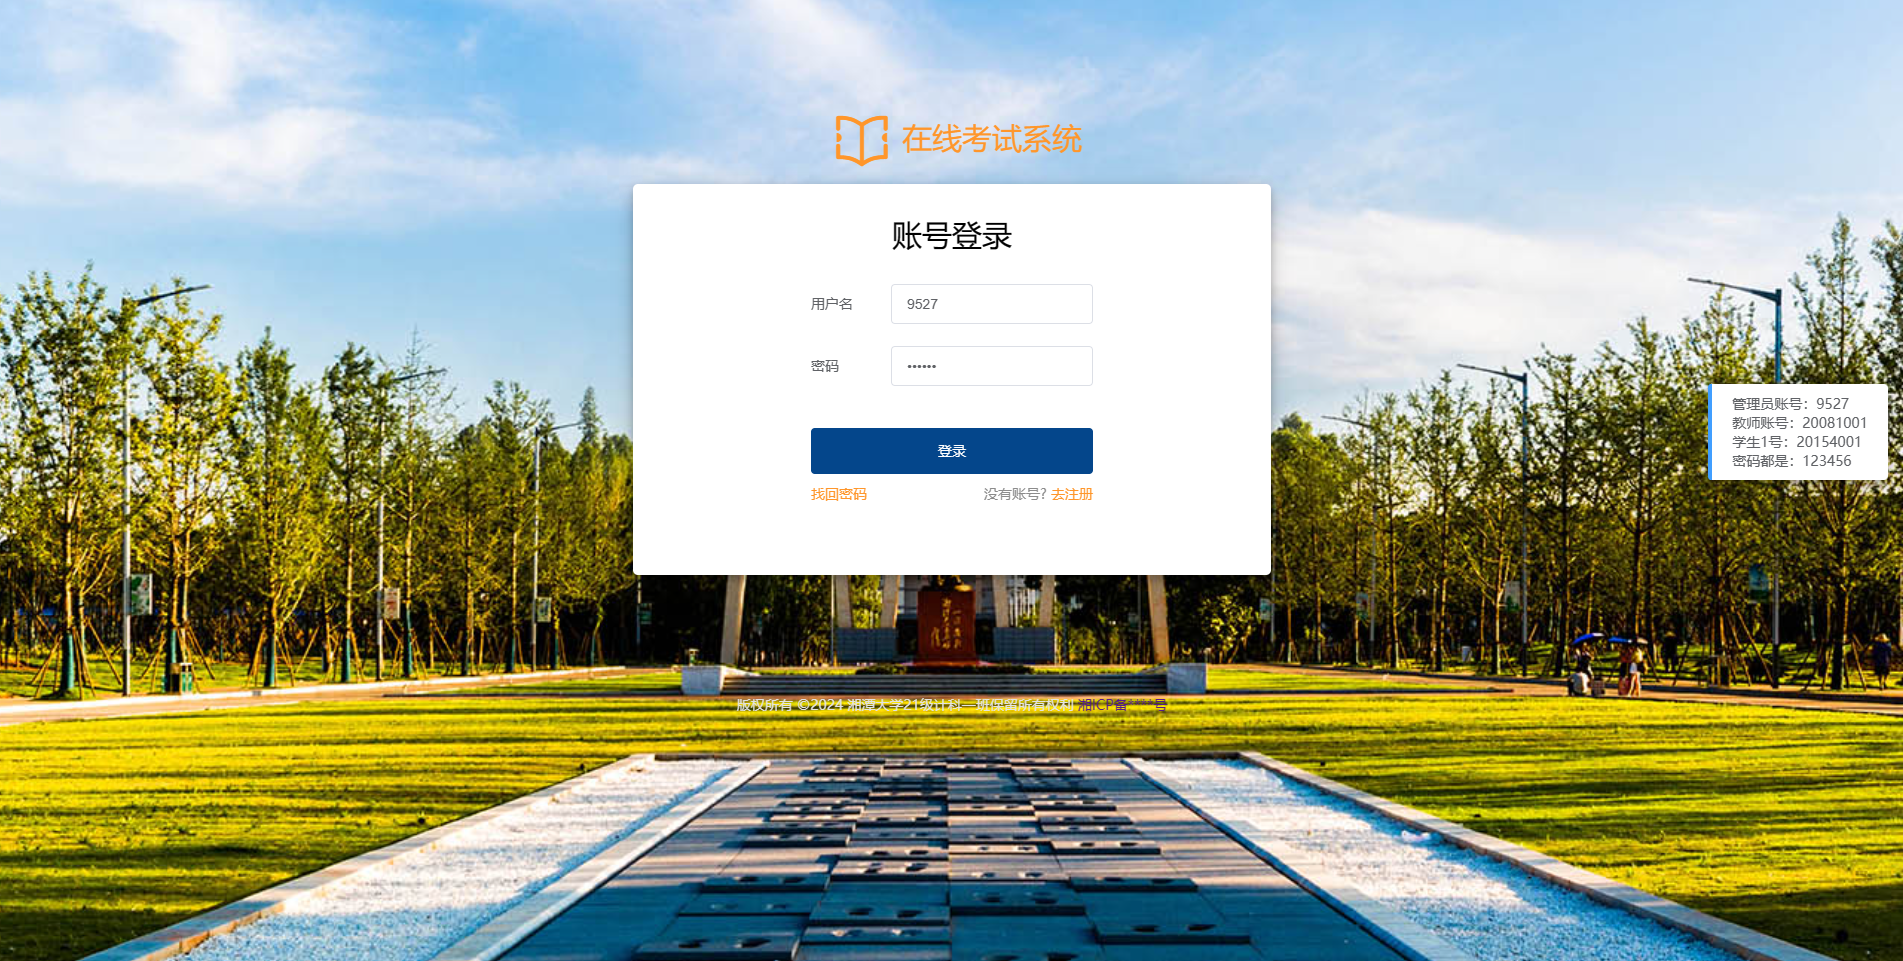
\includegraphics[width=0.75\linewidth]{1.png}
\end{figure}
\end{frame}

\begin{frame}[fragile]{功能展示}
\framesubtitle{添加试题}
\begin{figure}
    \centering
    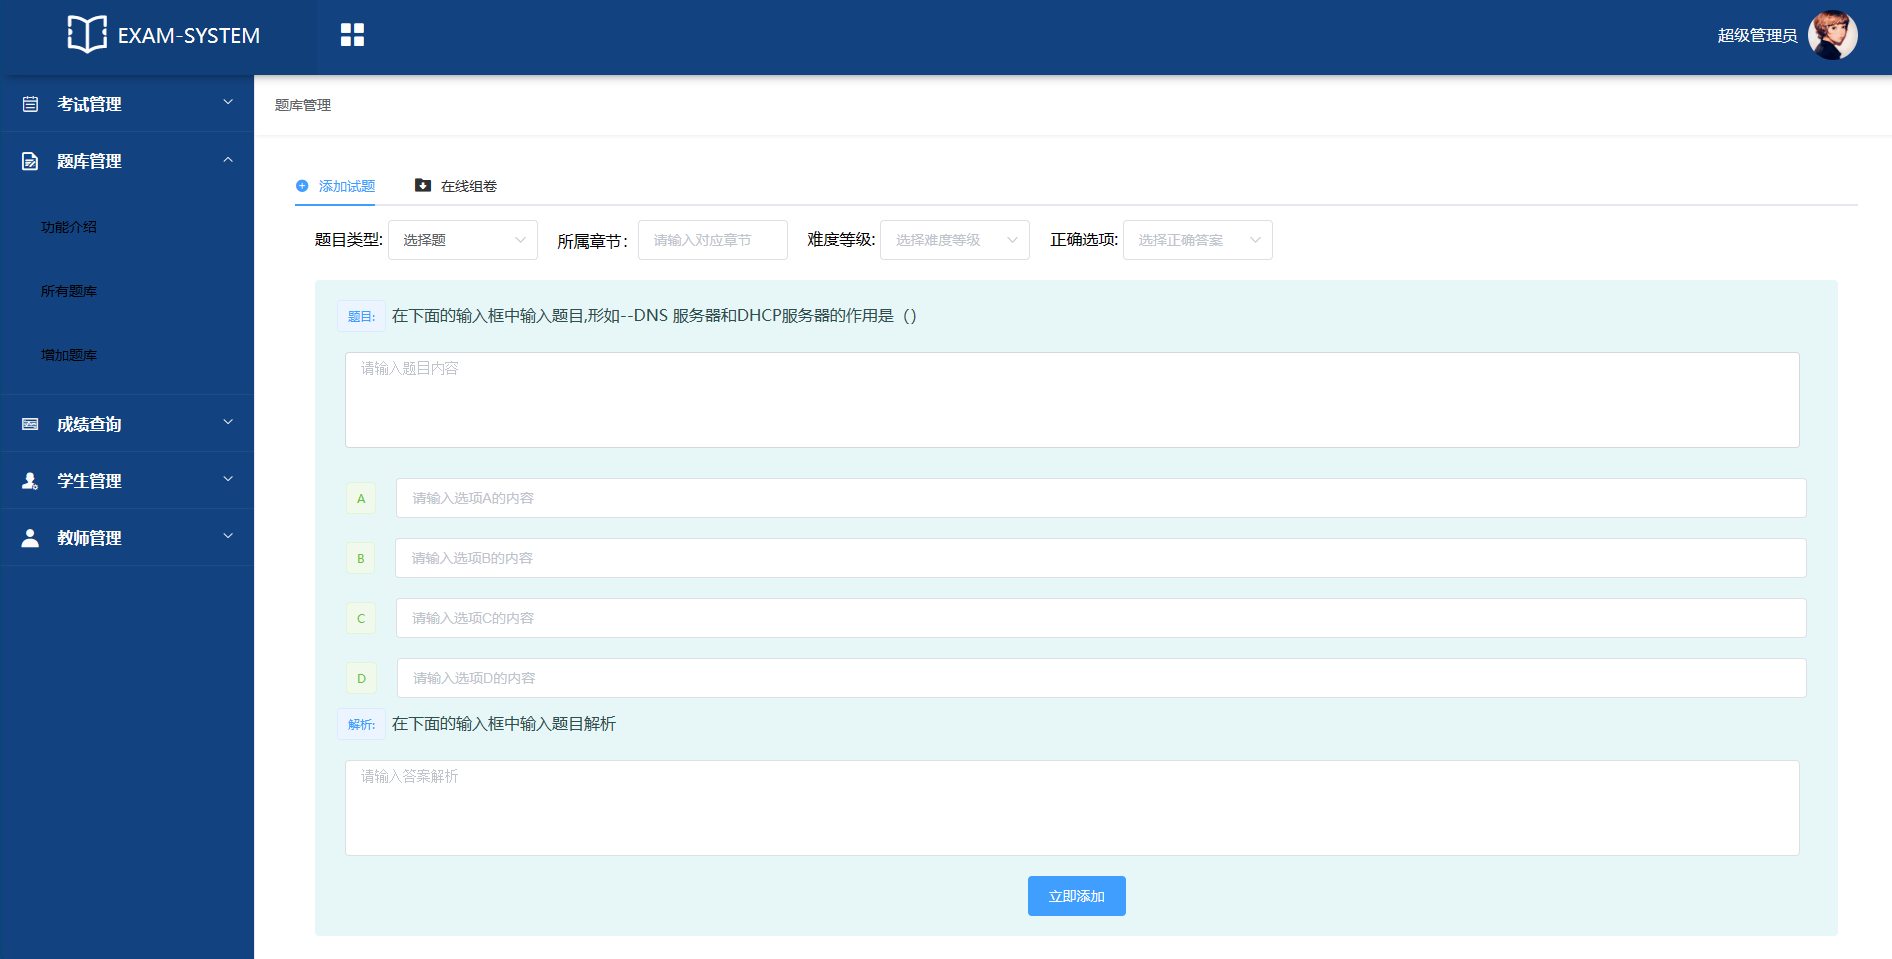
\includegraphics[width=0.75\linewidth]{2.png}
\end{figure}
\end{frame}

\begin{frame}[fragile]{功能展示}
\framesubtitle{考试查询}
\begin{figure}
    \centering
    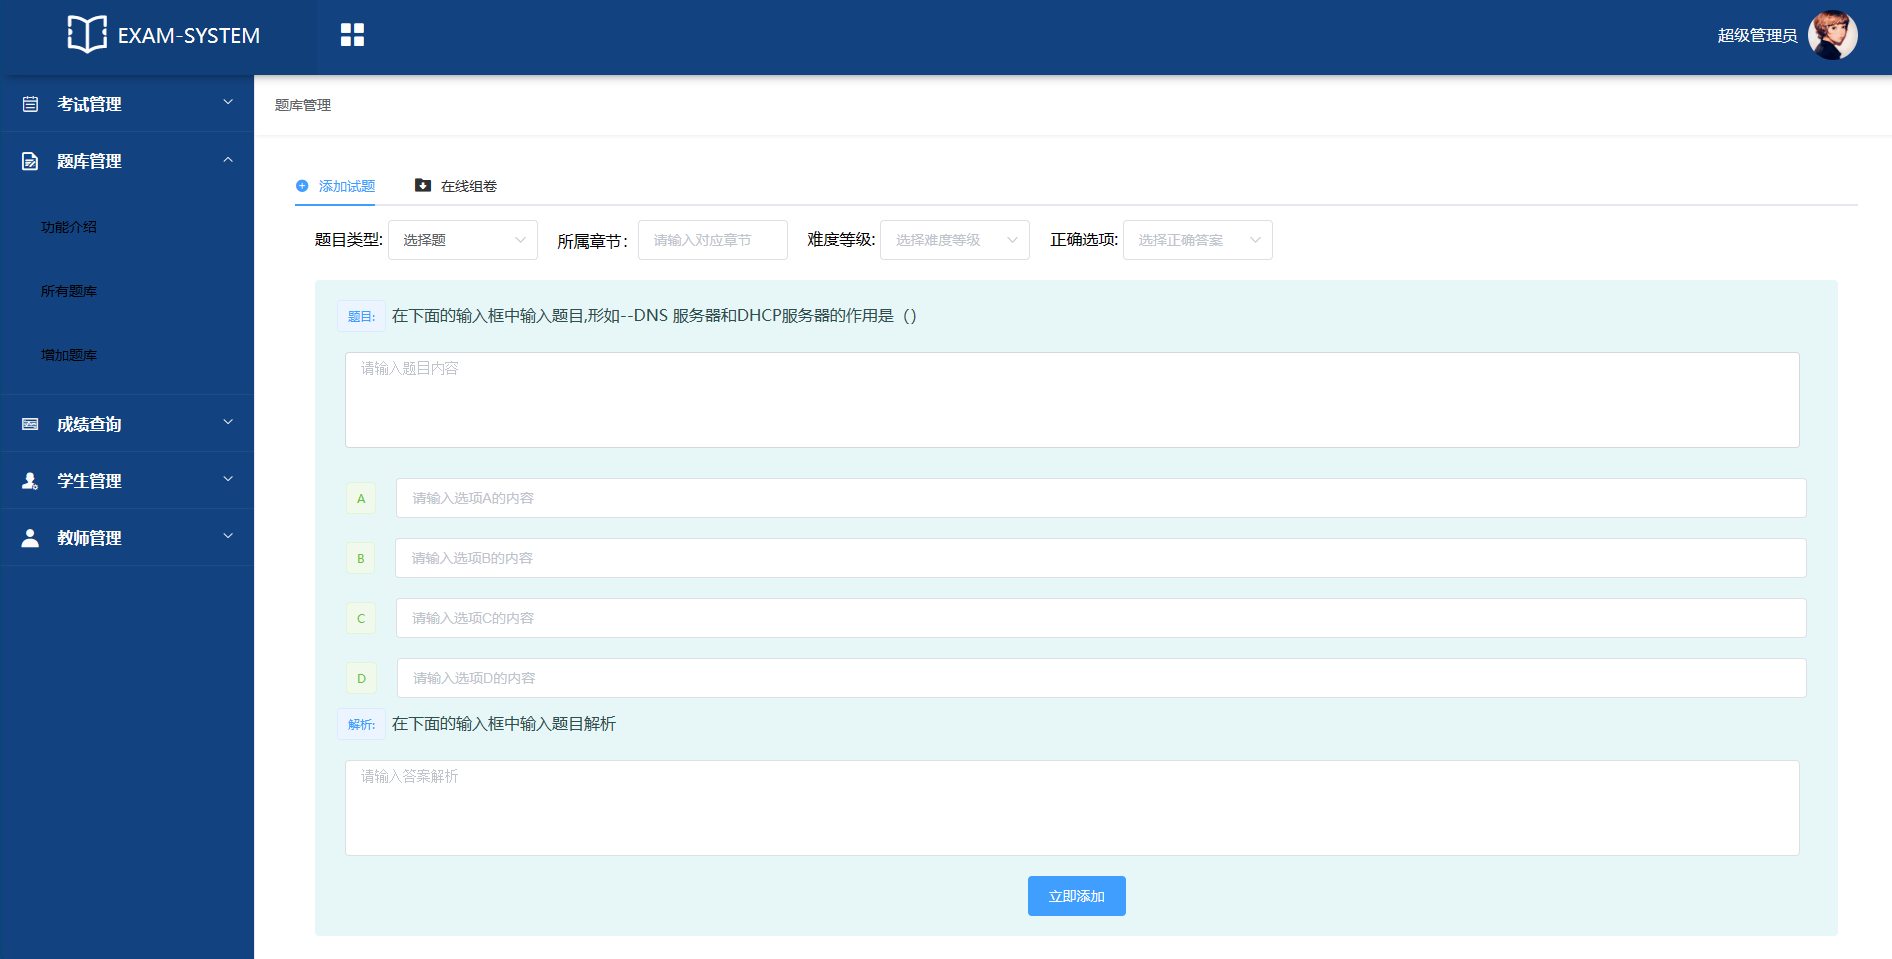
\includegraphics[width=0.75\linewidth]{2.png}
\end{figure}
\end{frame}

\begin{frame}[fragile]{功能展示}
\framesubtitle{试卷列表}
\begin{figure}
    \centering
    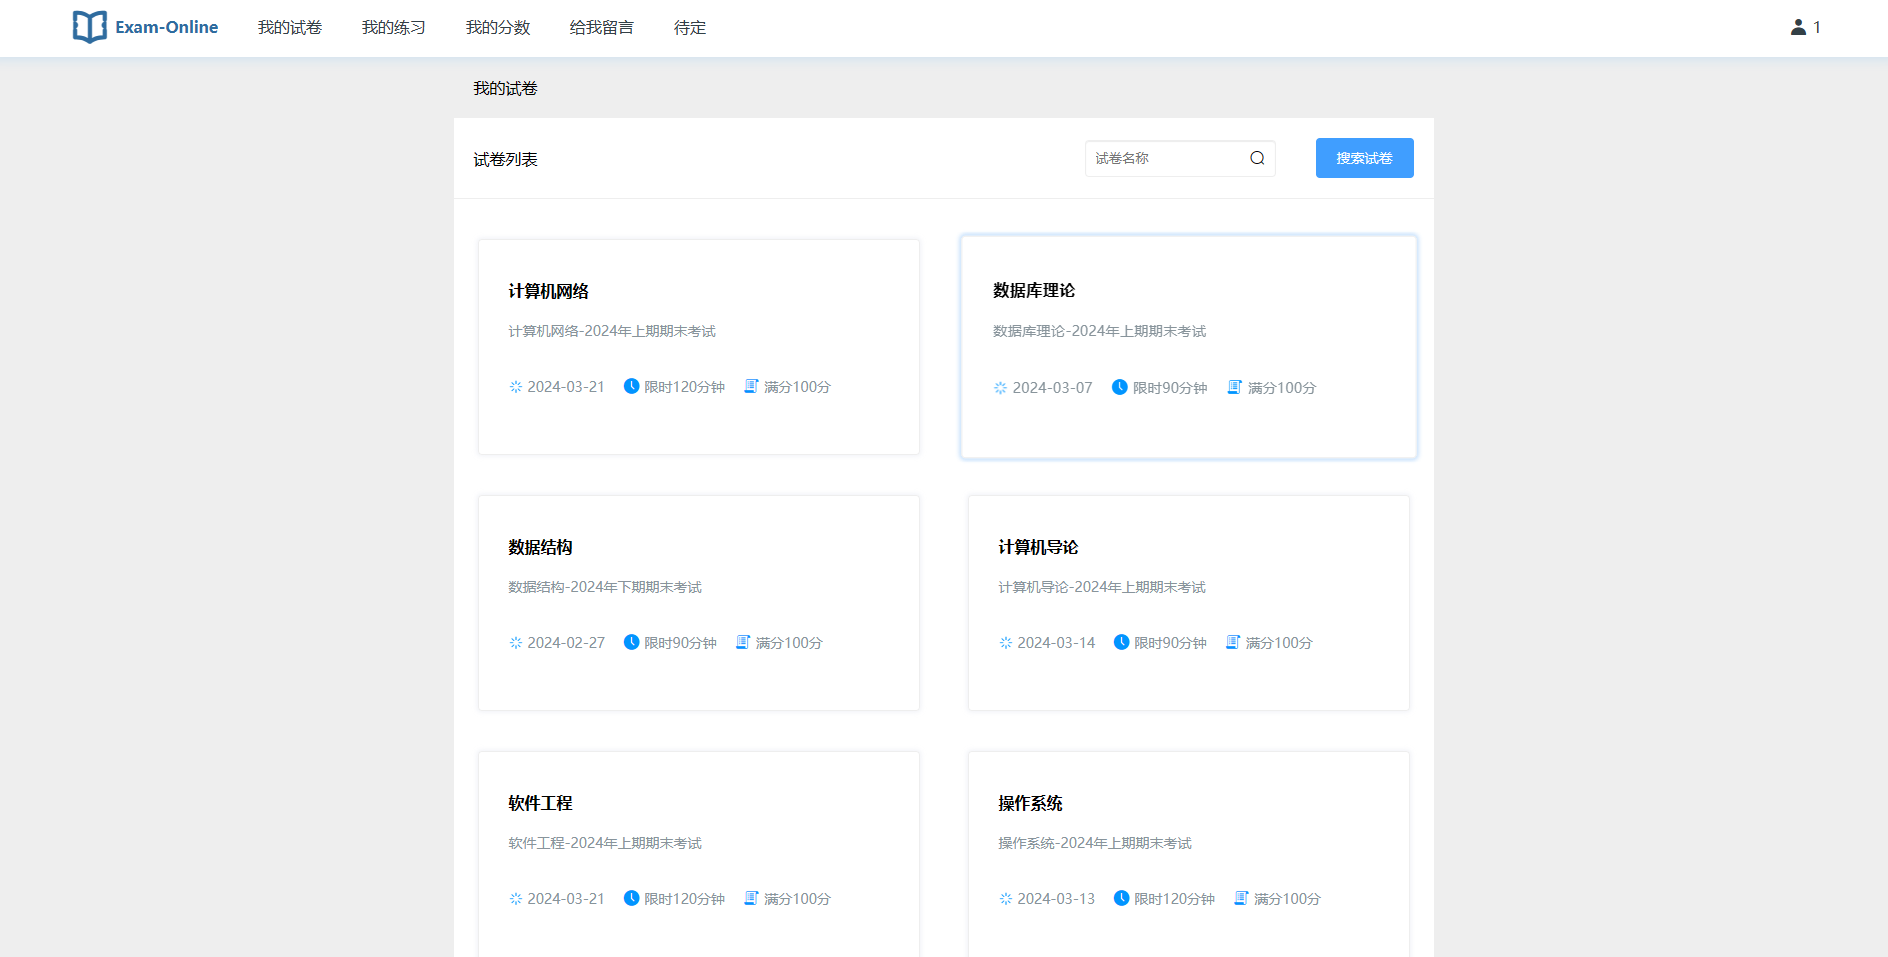
\includegraphics[width=0.75\linewidth]{4.png}
\end{figure}
\end{frame}

\begin{frame}[fragile]{功能展示}
\framesubtitle{查询学生分数}
\begin{figure}
    \centering
    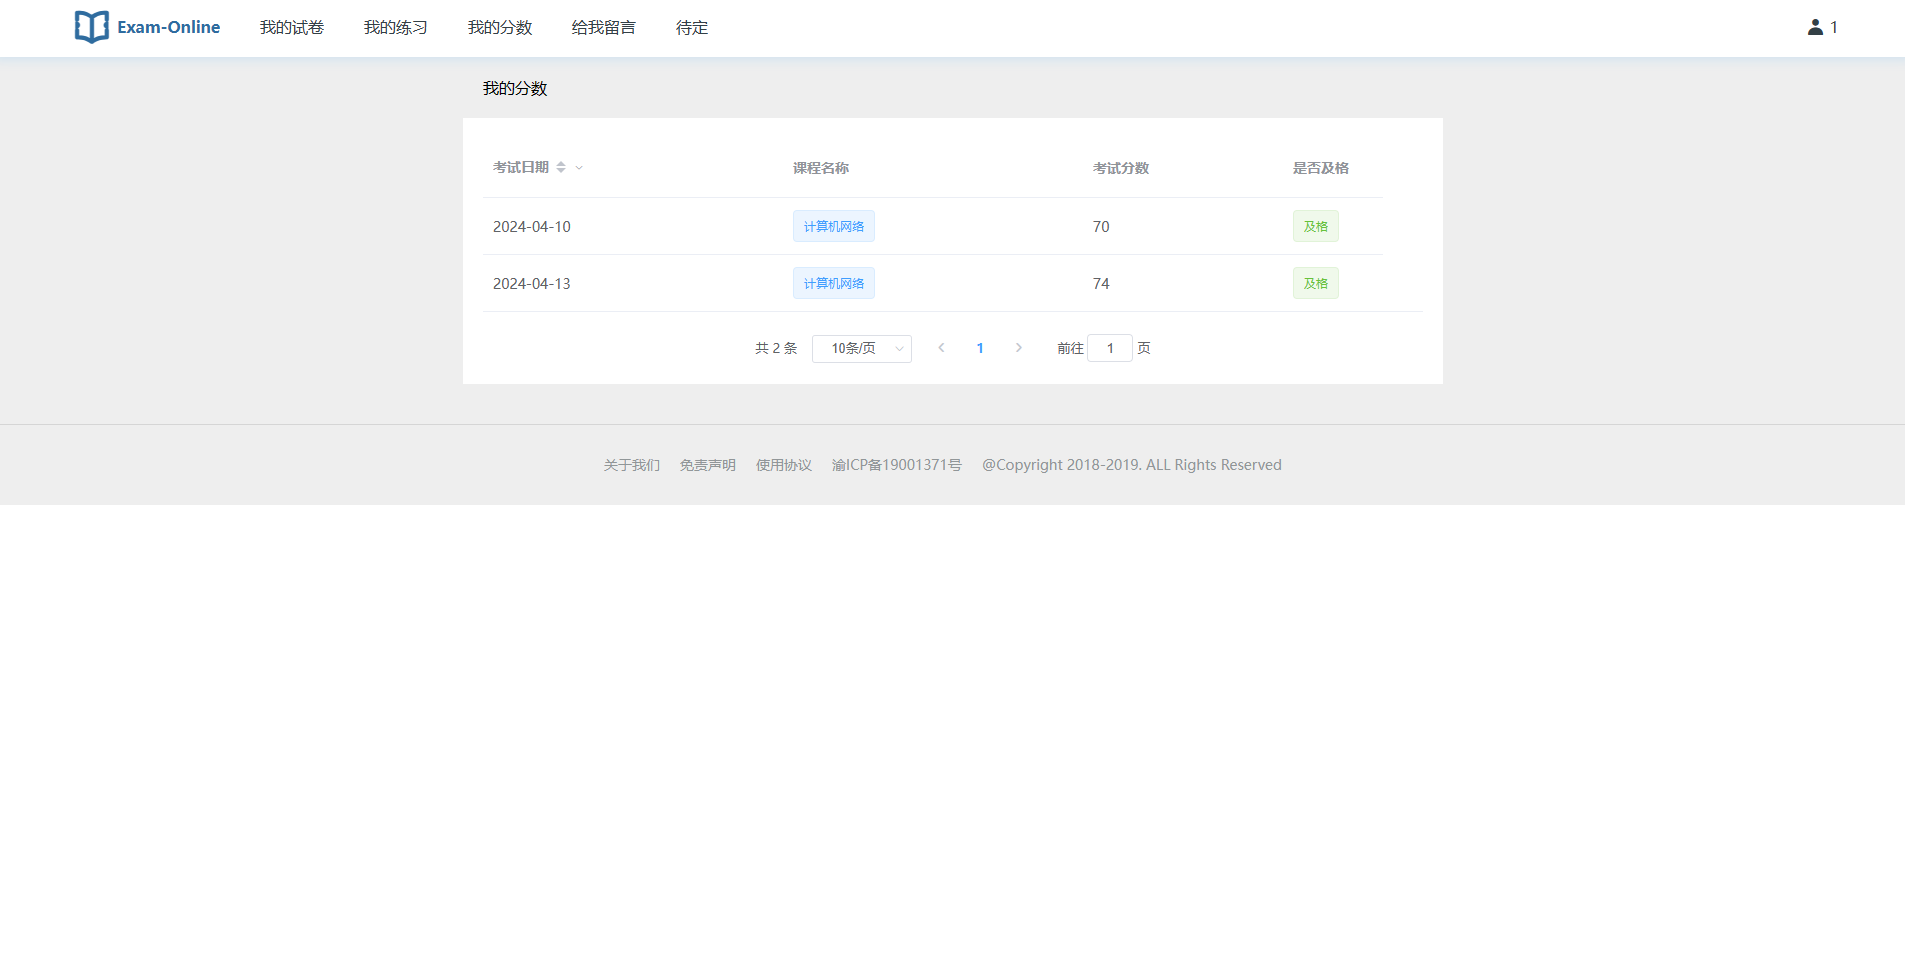
\includegraphics[width=0.75\linewidth]{5.png}
\end{figure}
\end{frame}

\backmatter
\end{document}
